\documentclass[12pt]{article}
\usepackage{graphicx}
\usepackage[margin=1in]{geometry}
\usepackage{caption}
\usepackage{xcolor}
\usepackage{float}
\usepackage{amsmath}
\usepackage{array}
\usepackage{multicol}
\usepackage{hyperref}
\usepackage{url}
\usepackage{listings}
\usepackage{courier}

\lstset{
  basicstyle=\ttfamily\footnotesize,
  backgroundcolor=\color{gray!10},
  frame=single,
  breaklines=true,
  captionpos=b
}

\setlength{\columnsep}{1cm}

\begin{document}

% Title Block
\begin{figure}[H]
    \begin{minipage}{0.45\textwidth}
        \includegraphics[width=\textwidth]{i.png} % <-- Replace with actual image
    \end{minipage} \hfill
    \begin{minipage}{0.45\textwidth}
        \textbf{Name: A. Likhitha} \\
        \textbf{Batch: COMETFWC019} \\
        \textbf{Date: 06 july 2025}
    \end{minipage}
\end{figure}

\begin{center}
    {\LARGE \textbf{\textcolor{cyan}{GATE 2009, EEE Question Number 13}}}
\end{center}
\vspace{1em}

\begin{multicols}{2}

\noindent\textbf{Abstract} \\[0.5em]
This project demonstrates the behavior of the NAND gate using  Pico2w, push buttons as logic inputs, and an LED to indicate output. It validates the concept that NAND is a universal gate.

\vspace{1em}
\noindent\textbf{1. Components}
\begin{table}[H]
\small
\centering
\begin{tabular}{|p{4.2cm}|c|}
\hline
\textbf{Component} & \textbf{Qty} \\
\hline
 Pico2w & 1 \\
Push Buttons & 2 \\
LED & 1 \\
220$\Omega$ Resistors & 3 \\
Breadboard & 1 \\
Jumper Wires & 10 \\
Laptop with Thonny IDE & 1 \\
\hline
\end{tabular}
\caption*{Table: Components used}
\end{table}

\vspace{1em}
\noindent\textbf{2. Setup Instructions}
\begin{itemize}
    \item Connect button A to GP14 with pull-down logic.
    \item Connect button B to GP15 similarly.
    \item Connect LED anode to GP13 through a 220Ω resistor.
    \item Common ground for both buttons and LED cathode.
    \item Use Thonny IDE to upload the code.
\end{itemize}

\vspace{1em}
\noindent\textbf{3. NAND Gate Logic}
\[
\text{NAND}(A, B) = \overline{A \cdot B}
\]
\[
\text{Output} = 
\begin{cases}
1 & \text{if } A = 0 \text{ or } B = 0 \\
0 & \text{if } A = 1 \text{ and } B = 1
\end{cases}
\]
\end{multicols}
\vspace{1em}
\noindent\textbf{4. Observation Table}
\\
\[
\begin{array}{|c|c|c|}
\hline
A & B & LED (Output) \\
\hline
0 & 0 & 1 \\
0 & 1 & 1 \\
1 & 0 & 1 \\
1 & 1 & 0 \\
\hline
\end{array}
\]

\vspace{19em}
\textbf{5. Circuit Image}\\ 
\\
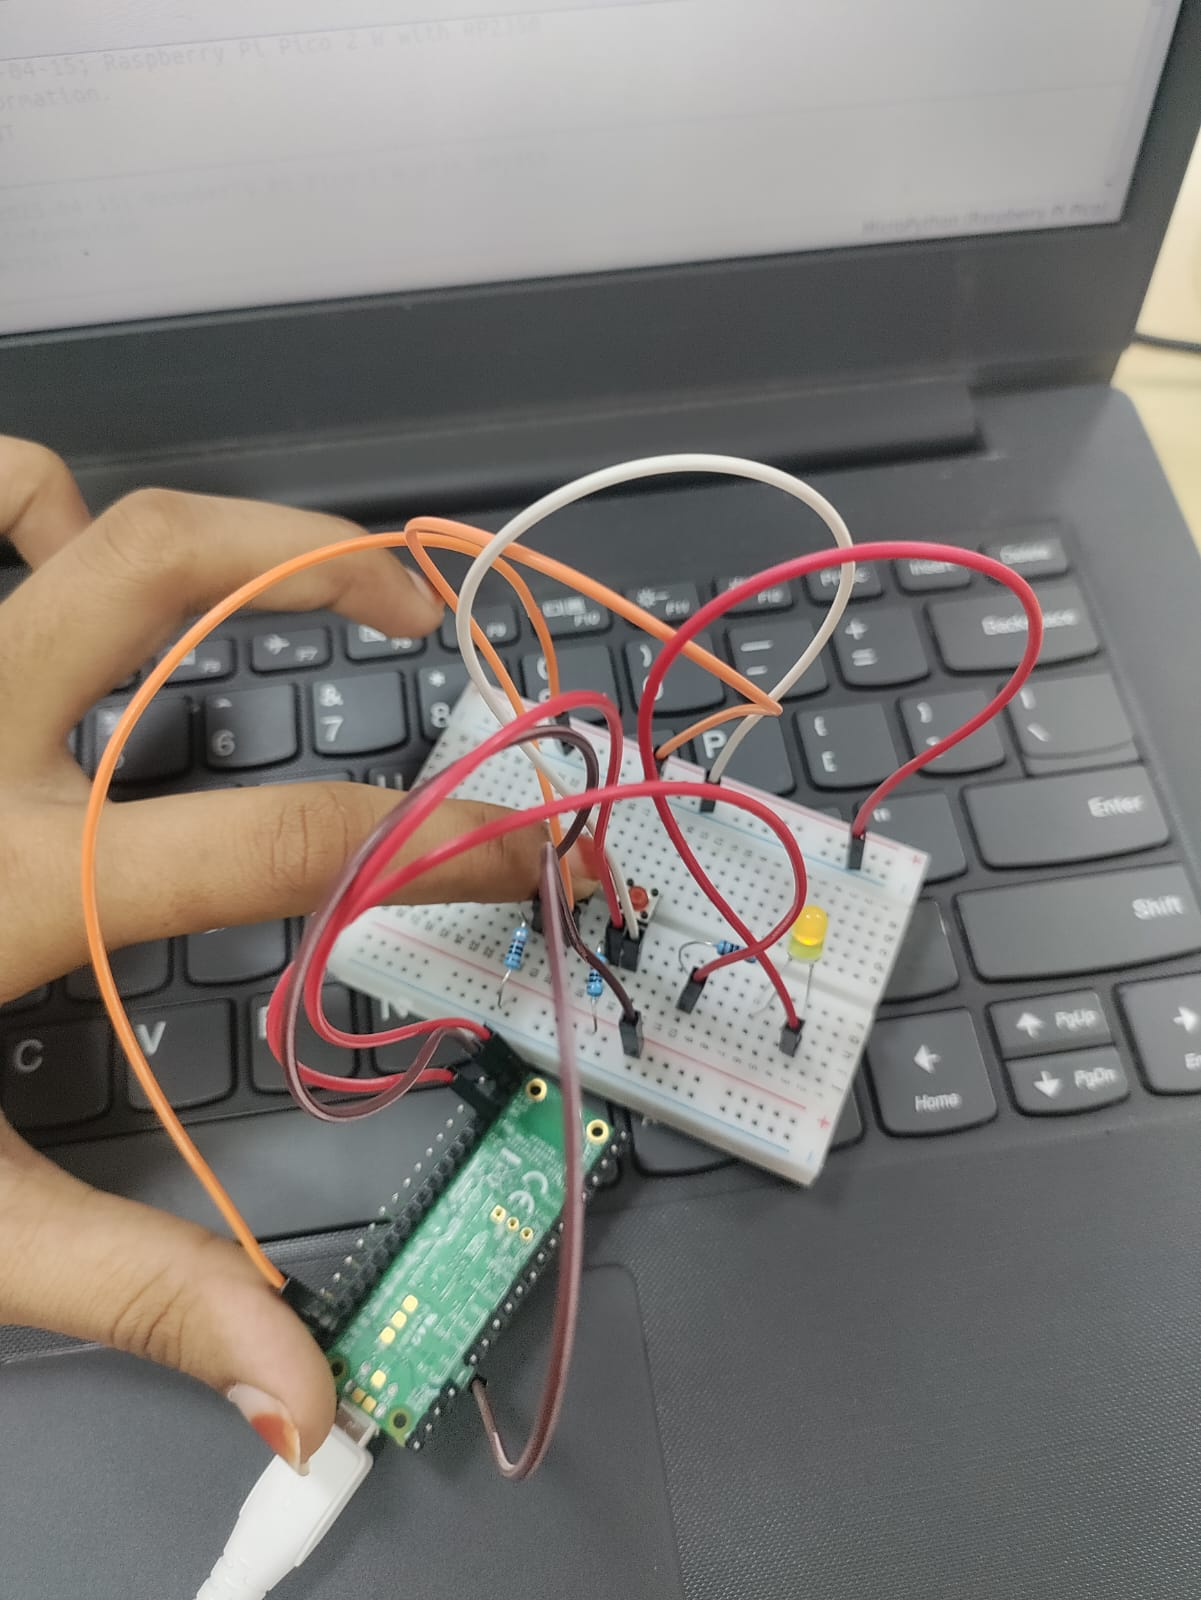
\includegraphics[width=0.6\linewidth]{output.jpeg} 


\vspace{1em}
\noindent\textbf{6. GitHub Code Link} \\
\url{https://github.com/amuru052004/Likhitha_fwc/tree/main/Hardware/platformio}

\vspace{1em}
\noindent\textbf{7. Conclusion}

This implementation verifies the behavior of a NAND gate using  Pico2w. 

\end{document}
